\subsection{phase vocoder}

    \begin{frame}{time stretching}{phase vocoder}
        \begin{enumerate}
            \item	\textbf{split input} signal into overlapping blocks
            \item<2->	compute \textbf{magnitude and phase spectrum} of each block
            \item<3->	\textbf{change overlap ratio} between blocks depending on stretch factor
            \item<4->	keep the magnitude, \textbf{adapt the phase per bin} to the block's new time stamp
        \end{enumerate}
        
        \begin{columns}
            \column{6cm}\vspace{-8mm}
                \begin{figure}
                    \begin{picture}(80,30)
                        \setcounter{iYOffset}{30}
                        \put(0, \value{iYOffset}){\tiny{\textcolor{gtgold}{input signal}}}
                        \setcounter{iXOffset}{0}
                        \addtocounter{iYOffset}{-3}
                        
                        \only<1->
                        {    
                            \put(\value{iXOffset}, \value{iYOffset}){\framebox(36, 2)}    

                            \addtocounter{iYOffset}{-2}
                            \setcounter{i}{1}
                            \whiledo{\value{i}<6}	
                            {
                                \put(\value{iXOffset}, \value{iYOffset}){\framebox(16, .5)}
                                \dottedline{.5}(\value{iXOffset}, \value{iYOffset})(\value{iXOffset},29)
                                \addtocounter{iXOffset}{5}
                                \addtocounter{iYOffset}{-1}
                                \stepcounter{i} 
                            }	
                        }
                        \only<2->
                        {    
                            \put(15,18){{$\Downarrow$}}
                            
                            \put(47,16){\ovalbox{\tiny{\parbox{20mm}{\centering{STFT\\ magnitude \& phase}}}}}
                        }
                        
                        \only<3->
                        {    
                            \setcounter{iXOffset}{0}
                            \setcounter{iYOffset}{14}
                            \setcounter{i}{1}                            
                            \whiledo{\value{i}<6}	
                            {
                                \put(\value{iXOffset}, \value{iYOffset}){\framebox(16, .5)}
                                %\dashline{4}(0,11)(60,11)
                                \dottedline{.5}(\value{iXOffset}, \value{iYOffset})(\value{iXOffset},2)
                                \addtocounter{iXOffset}{7}
                                \addtocounter{iYOffset}{-1}
                                \stepcounter{i} 
                            }	
                            \addtocounter{iYOffset}{-3}
                        }
                        \only<4->
                        {    
                            \put(15,6){{$\Downarrow$}}
                            \put(47,6){\ovalbox{\tiny{\parbox{20mm}{\centering{phase extrapol. \\ window comp.}}}}}
                        }
                        
                        \only<5->
                        {    
                            \put(0, 2){\framebox(44, 2)}    
                            \put(0, 0){\tiny{\textcolor{gtgold}{output signal}}}
                        }
                    \end{picture}
                \end{figure}

            \column{4cm}\vspace{-20mm}
                    \vspace{20mm}
                \only<4>
                {
                     \begin{figure}
                        \centering
                        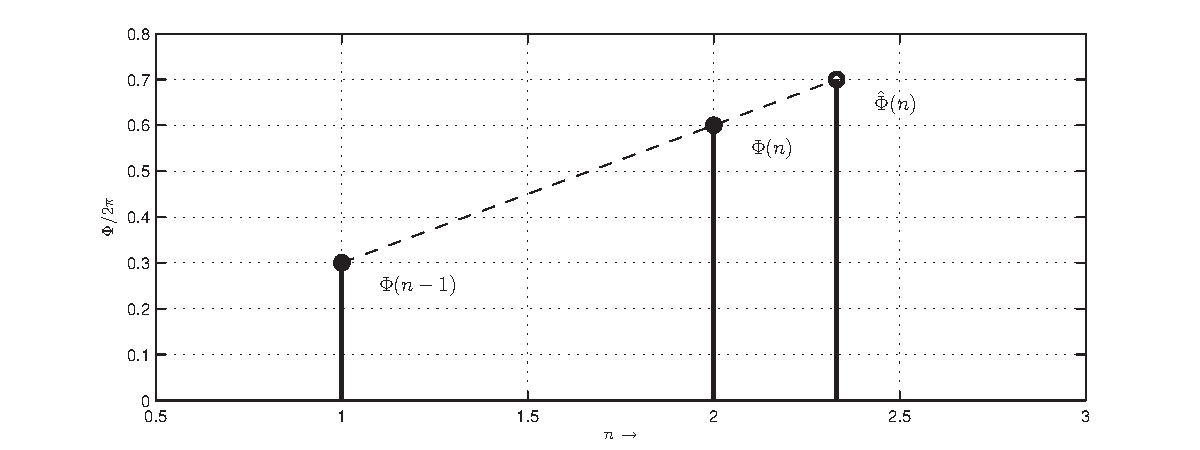
\includegraphics[scale=.25]{graph/phaseextrapol.pdf}
                     \end{figure}
                }
                \only<5->
                {
                    \begin{itemize}
                        \item   original \includeaudio{audio/cathy.mp3}
                        \item   pv $s = \nicefrac{4}{3}$ \includeaudio{audio/cathypvout.mp3}
                    \end{itemize}
                }
        \end{columns}
        \vspace{50mm}
    \end{frame}

    \begin{frame}\frametitle{time stretching}\framesubtitle{phase vocoder window compensation}
        \begin{figure}
            \centerline{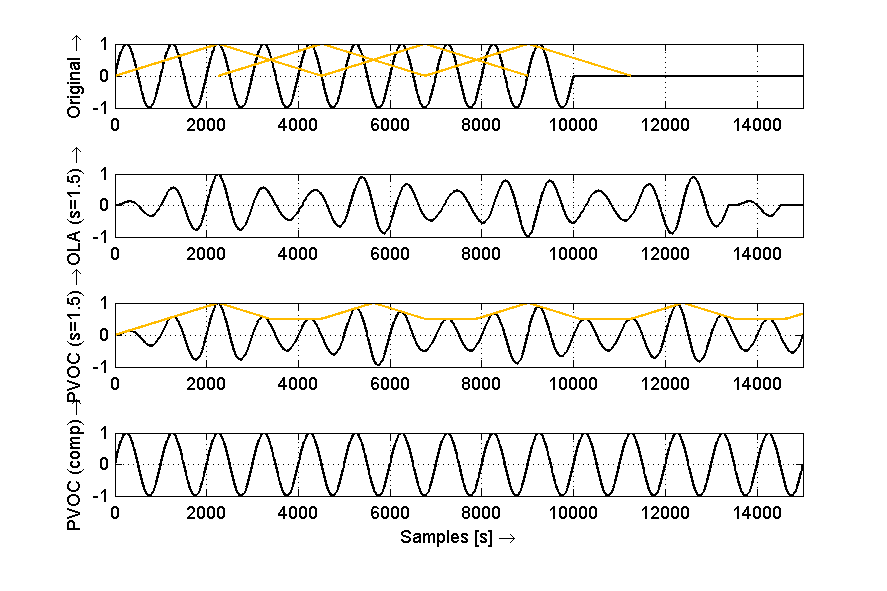
\includegraphics[scale=.7]{graph/pvocIntro}}
        \end{figure}
    \end{frame}

    %\begin{frame}\frametitle{time stretching}\framesubtitle{phase vocoder phase unwrapping}
        %ENTER PHASE UNWRAPPING INFO HERE
    %\end{frame}

    \begin{frame}{time stretching}{phase vocoder --- properties \& artifacts}
        \begin{itemize}
            \item   \textbf{advantages}:
                \begin{itemize}
                    \item   allows \textit{polyphonic input} (assumption: no overlapping harmonics)
                    \item   absolute \textit{timing stability} (i.e., sample resolution)
                \end{itemize}   
            \pause
            \bigskip
            \item   \textbf{disadvantages}:
                \begin{itemize}
                    \item   \textit{low granularity} --- FFT block size
                    \item   artifacts:
                        \begin{enumerate}
                            \item   phasing
                            \item   transient smearing/doubling
                        \end{enumerate}
                \end{itemize}
        \end{itemize}
    \end{frame}

    \begin{frame}{time stretching}{phase vocoder artifacts: phasing --- spectral leakage 1/3}
            \begin{figure}
                \centering
                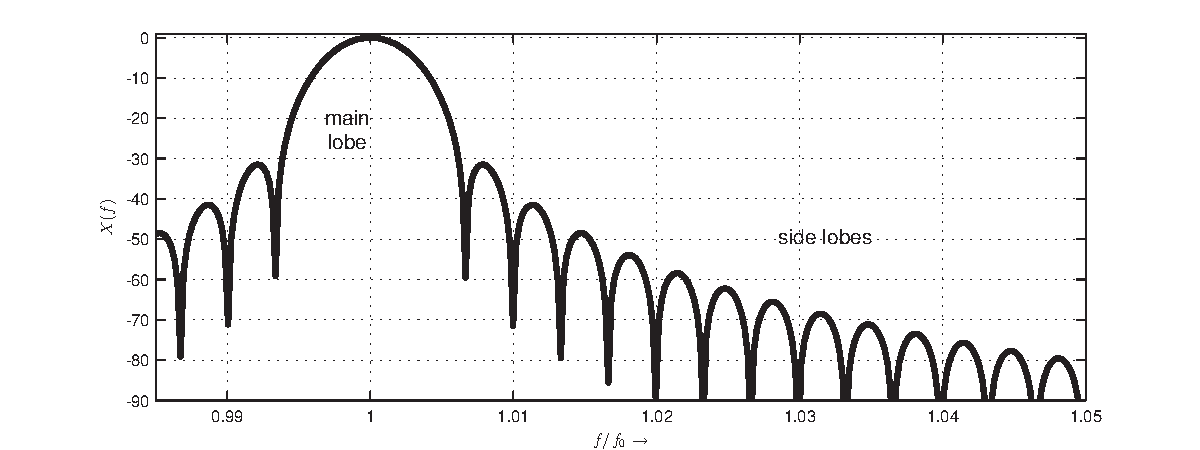
\includegraphics[scale=.3]{graph/SpectralLeakage}
            \end{figure}
            \begin{figure}
                \centerline{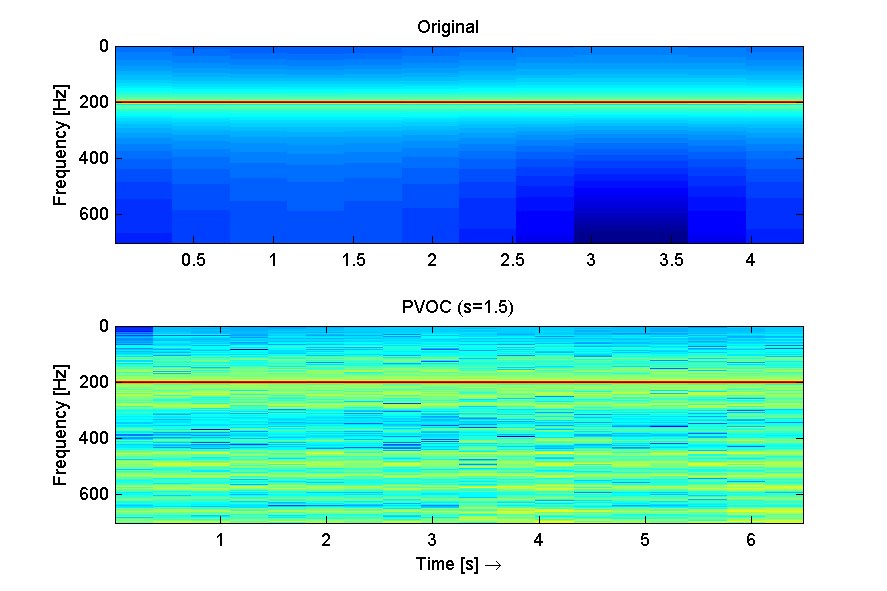
\includegraphics[scale=.5]{graph/PeakSmearingFreq}}
            \end{figure}
    \end{frame}
	\begin{frame}{time stretching}{phase vocoder artifacts: phasing --- spectral leakage 2/3}
			\begin{figure}
				\centerline{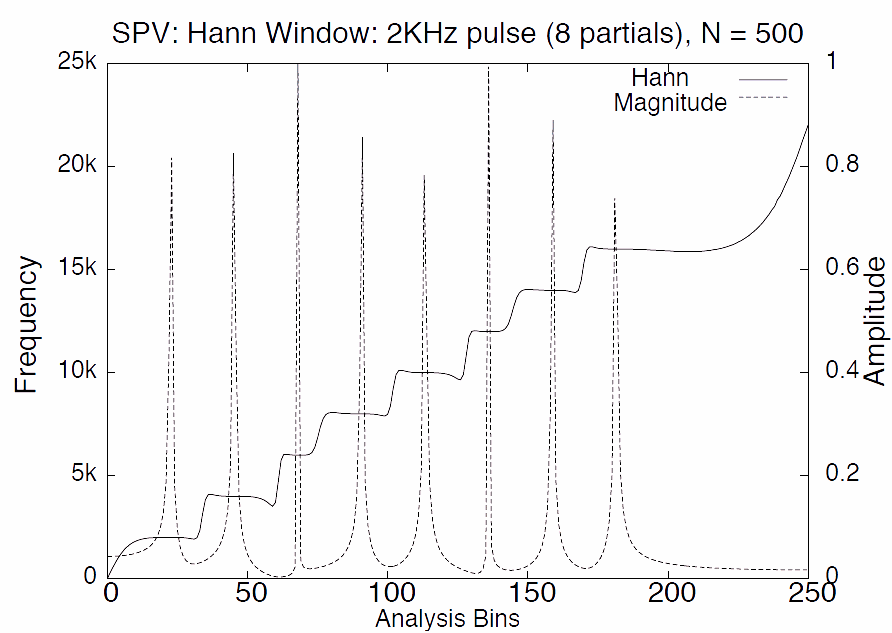
\includegraphics[scale=.4]{graph/instfreq}}
			\end{figure}
    \end{frame}
	\begin{frame}{time stretching}{phase vocoder artifacts: phasing --- spectral leakage 3/3}
                \begin{itemize}
                    \item[$\Rightarrow$] use \textit{frequency reassignment} for grouping and phase sync
                \end{itemize}
                \bigskip
                        \begin{itemize}
                            \item   original  \includeaudio{audio/cathy.mp3}
                            \item   pv $s = \nicefrac{4}{3}$ \includeaudio{audio/cathypvout.mp3}
                            \item   grouped phase \includeaudio{audio/cathyEffout.mp3}
                        \end{itemize}
    \end{frame}
	\begin{frame}{time stretching}{phase vocoder artifacts: phasing --- unsynced harmonics}
                        \begin{figure}
                            \centering
                                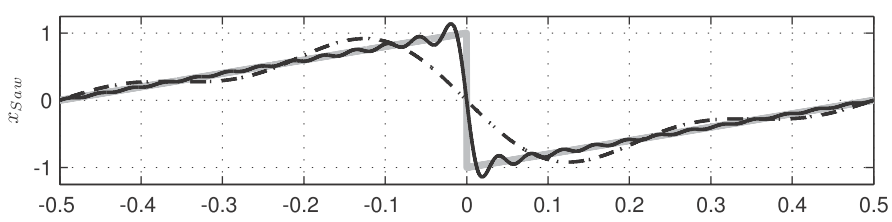
\includegraphics[width=5.3cm,height=2.4cm]{graph/gibbs}
                        \end{figure}
		\only<1>{
		\begin{figure}
			\centerline{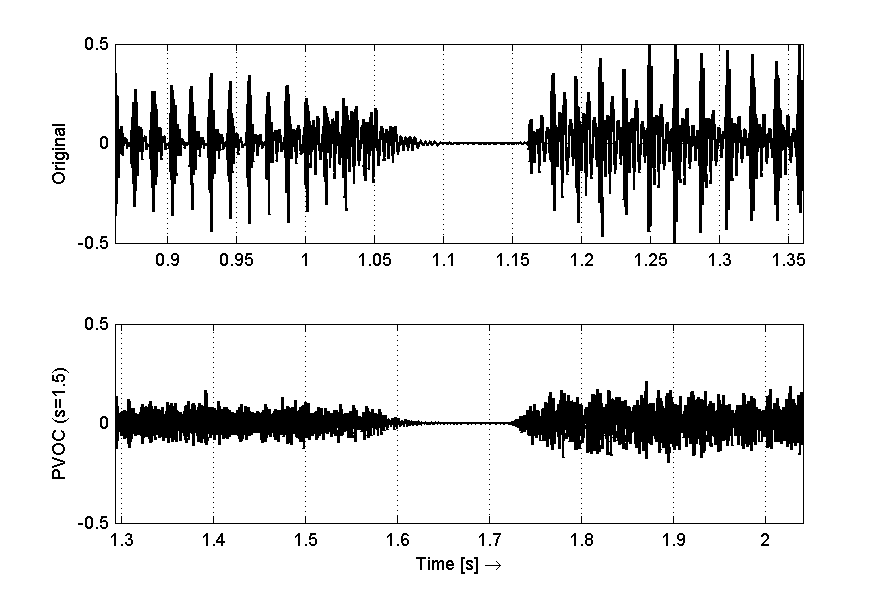
\includegraphics[scale=.5]{graph/phasing}}
		\end{figure}}
        \pause
                \begin{itemize}
                    \item[$\Rightarrow$] use \textit{harmonic analysis} for grouping and phase sync
                \end{itemize}
                        \begin{itemize}
                            \item   original  \includeaudio{audio/cathy.mp3}
                            \item   pv $s = \nicefrac{4}{3}$ \includeaudio{audio/cathypvout.mp3}
                            \item   synced phase \includeaudio{audio/cathyProout.mp3}
                        \end{itemize}
        \vspace{50mm}
    \end{frame}
	\begin{frame}{time stretching}{phase vocoder artifacts: interchannel phasing}
        \begin{itemize}
            \item   phase estimation between channels slightly off due to
                \begin{itemize}
                    \item   numerical inaccuracies (cumulative!)
                    \item   overlapping frequency components
                \end{itemize}
                \pause
                \bigskip
            \item[$\Rightarrow$] change in spatial image
                \begin{itemize}
                            \item   original  \includeaudio{audio/bigband.mp3}
                            \item   pv $s = \nicefrac{3}{2}$ \includeaudio{audio/bigbandPVoc.mp3}
                \end{itemize}
        \end{itemize}
	\end{frame}

    \begin{frame}{time stretching}{phase vocoder artifacts: transient smearing}
        \vspace{-5mm}
        \begin{columns}
            \column{.65\textwidth}\vspace{-5mm}
                \begin{figure}
                    \centering
                    \includegraphics[scale=.35]{graph/TransientSmear}
                \end{figure}\vspace{-5mm}

            \column{.3\textwidth}%\vspace{-10mm}
                \begin{itemize}
                    \item   original  \includeaudio{audio/castanets.mp3}
                    \item   pv $s = \nicefrac{3}{2}$ \includeaudio{audio/castanetsPVoc.mp3}
                \end{itemize}
        \end{columns}
        \pause
        \begin{itemize}
            \item[$\Rightarrow$] detect transients and \textit{reset phase} per bin
        \end{itemize}
                \begin{itemize}
                    \item   original  \includeaudio{audio/41_m.mp3}
                    \item   pv $s = \nicefrac{4}{3}$ \includeaudio{audio/41pvout.mp3}
                    \item   phase reset \includeaudio{audio/41Proout.mp3}
                \end{itemize}


    \end{frame}

\begin{frame}\frametitle{time stretching}\framesubtitle{inherent problems}
	\begin{itemize}
		\item	stretching the audio data can lead to \textbf{``non-natural'' results}
		\pause
        \bigskip
		\item	\textbf{examples}
			\begin{itemize}
				\item tempo dependent \textit{timing variations }
				\pause
				\item	other performance related aspects may get inappropriate lengths and speed: \textit{vibrato, tremolo, glissando}
			\end{itemize}
	\end{itemize}
\end{frame}
